% Section content template for individual Educative lessons
% This file contains the actual content for a specific section
% Generated from Educative API section content

% Section: Activity Diagram for ESPNcricinfo
% Section ID: 5446998141698048
% Section Slug: activity-diagram-for-espncricinfo
% Generated: 2025-12-14T13:33:26.633446

Activity diagrams are an effective way to visualize the flow of messages between activities within a system. We can create different activity diagrams for ESPNcricinfo. In this lesson, we will create an activity diagram to record the movement of a ball.

\subsection{Make a record of a ball}\label{R3xHl--qa8e-0GwZ3M4M_}
\\
The states and actions involved in this activity diagram are provided below.

\subsubsection{States}\label{JlKCald8UdxMpgz6tk--G}
\\
\textbf{Initial state:~} The system adds a ball to the over.
\\
\textbf{Final state:}~The ball record is saved.

\subsubsection{Actions}\label{1MkRFl9Y-yBLTzREphGbG}
\\
The system adds a ball to the over, choosing the ball type that was bowled. It determines if the batter got out. If they did not, it adds to the score that was made. Finally , the commentary is added to the ball, and the ball record is saved.

\begin{figure}[htbp]
 \centering
 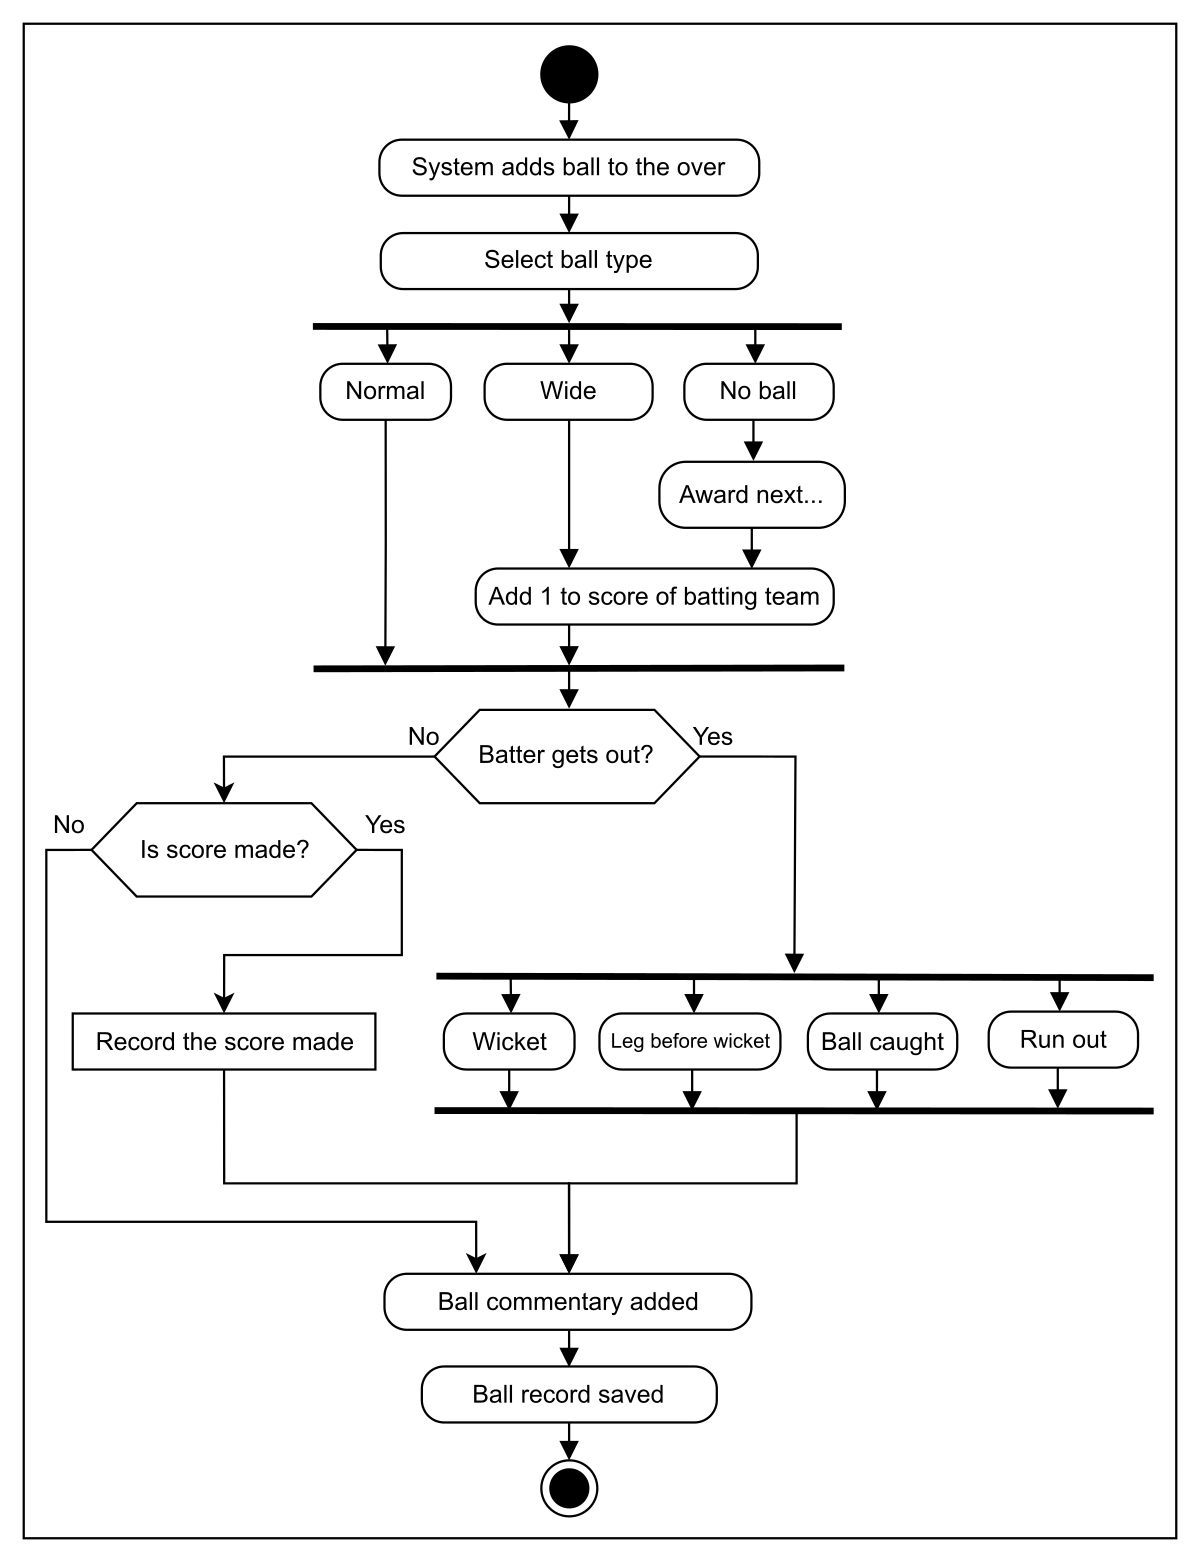
\includegraphics[width=0.5\textwidth]{Images/chapter_26/section_5446998141698048/5219635178635264.png}
 \caption{The activity diagram for making a record of a ball}
\end{figure}

In the next lesson, we will present the code for our designed classes in some of the most popular languages.

% End of section content